\begin{savequote}[75mm]
A new life awaits you in the Off-world colonies! A chance to begin again in a golden land of opportunity and adventure!
\qauthor{Blade Runner}
\end{savequote}

\chapter{A hypermedia model of the user on\hyph line footprint}

\newthought{Web services} use personal data to sustain their business by fuelling this stream of information to recommendation systems to generate tailored advertising. When users decide to subscribe a service, they automatically lose control over the data generated by their activity. This is especially true when third parties are authorised to access a user's profile and information. This is often the case of mobile and web application implementing their log-in flow through a larger authorisation provider, like Google or Facebook. We introduce a hypermedia model of the user online footprint and present a privacy broker allowing users to retain control on their data. Our defined model can be both used to transfer data between services and clients and to express the value and risk of sharing certain information.

\section{Background}

The business model of many services and applications on today's web is based on having user authenticate and, completely or partially, generate data to \emph{pay} for the possibility to use the service. Data is, in fact, used as a currency that can be resold for a variety of purposes. To target the users and suggest back product that they can buy, or to continuously track them across different visits, and in some cases different devices and websites.

Web services can furthermore dispose of the data collected as their property, as when users access a service they lose control and rights over their digital footprint. One of the problem associated with this is certainly linked to consent. Users give their implicit consent to the use of their data and subsequently their footprint, sometimes only in part, become property of the company providing the services. The same process of giving consent or granting permissions to access part of the user identity is not clear. This scenario is particularly evident when mobile applications request access to some resources on a user's phone, or when Facebook federated log-in mechanism is used. Facebook log-in provides both authentication and authorisation. The mechanism is used on the web as well as on iOS and Android, although on those platforms the primary mechanism uses the native Facebook application instead of the web API. When an application is connected to the user's Facebook profile using Facebook log-in, it can always access their \emph{public profile} information. Facebook consider this information public and will not apply any restriction on it. Information that is shared with the public profile vary from user to user and depends on their privacy settings. By default, the Facebook public profile includes some basic attributes about the person such as the user's age range, language and country, but also the name, gender, username and user ID (account number), profile picture, cover photo and networks. This is the minimum set of data disclosed by Facebook when the social network log-in mechanism is used to gain access to an app or service. This data is acquired by the app and user control over it is practically lost, as it will be disposed according to the app privacy policy.

We propose a model of the user identity and a privacy management system amd we introduce two possible examples. One is based on the WebSocket protocol and shows a handshake based on the Socialist Millionaires protocol. The second example is based on the OAuth 2.0 flow which uses JWT to transmit private information to third parties. This approach is similar, and builds upon, previous techniques, such as Crypto-Book~\cite{maheswaran2013crypto} and UnlimitID~\cite{isaakidis2016unlimitid}, using the technique of blacklistable anonymous credentials~\cite{tsang2007blacklistable}. The idea behind these techniques is that a trusted (or semi trusted) Identity Provider (IdP) issues an anonnymous credential $C(x)$ encoding a secret identity key x, unique and only known by the specific user. The user holding C(x) authenticates to a Service Provider (SP) by, given a cryptographically secure hash function and a secure elliptic curve group, producing a ticket $T$ depending on $x$, together with a zero-knowledge proof stating that they actually hold a valid credential from the IdP, the key used to compute $T$ is the same as their secret identity key used to comute $C(x)$ and no previous ticket associated with past abuses used the identity key $x$.

The following protocol allows the user to authenticate anonymously to the SP and eventually disclose private information with the same SP or third-parties as they please. We would like to stress that no modification is needed for existing web protocols or clients and that we make use of existing and widely adopted authorisation and authentication mechanism. Furthermore, the proposed hypermedia model allows the user to explore the shared preferences and properties shared with each service.

\section{A hypermedia model of the user identity}

Users interact with web services and applications with hypermedia protocols. Each time an action is completed onto an user's phone a call is performed to an APIs updating the user profile or sending some information to a service. These interactions are often completed over a REST protocol, such as HTTP, and consist of the client sending structured information to the server. This information can be anything regarding the user or the state of the used application, such as profile information or answers to specific queries initiated implicitly or explicitly by the user.

We define a model of the user identity to describe how a privacy policy can interact with data and which data or resource a service can access. Our model is based on the assumption that user data can be represented with a hypermedia object. This specifically mean that accessing a resource at a given time or accessing identification information opens up access to data connected to that resource or that identification. We begin by defining the identity model using JSONApi~\cite{Jsonapi} a specification for exchanging data between REST interfaces defining how a client should request that resources or their representations be fetched or modified, and how a server should respond to those requests. We envision that the same format can be used on the client side to represent identities and data associated with it and on the server side to request and exchange data.

\lstset{caption={Some user identity data encoded with JSONApi.},label=lst:JSONIdentity}
\begin{lstlisting}
{
    "data": {
        "type": "identity",
        "id": "john@johnsmith.com",
        "attributes":
            { // Attribute list },
        "relationships":
                { // Relationship list },
        "links": { // Third-party links }
    },
    "included": [ {
        "type": "resource",
        "id": "CC76598TDZKG9EEC3", // Device hardware id
        "attributes": { // resource attributes }
        "meta": { // Any meta information },
    }],
}
\end{lstlisting}

We model the user's activity as series of events belonging to a certain identity. Each event is a document containing different information. We can formally define this an hypermedia document i.e. an object possibly containing graphics, audio, video, plain text and hyperlinks. We call the hyperlinks selectors and we use these to build the connections between the user's different identities or events. Each identity is a profile that the user has created onto a service or platform. This can be an application account or a social network account, such as their LinkedIn or Facebook unique IDs.

Each event is the result of the user performing an action. For the purpose of this study we have consider an action as resulting using an application or a service. An action is the activity of interacting with a mobile application or \emph{liking} a resource on a social network, i.e. directly expressing an interest, or the fact that a user has updated their location at a certain time.

We find that this model is able to express the user's online footprint as a collection of traces left across different services. Furthermore, by using a hypermedia approach we are able to grasp the connections between the different profiles and features. This results in the possibility to profile users based on chosen selectors. For example, we might want to trace all users who have been in the radius of 500 meters to a certain location, or all the users in a certain neighbourhood who \emph{like} a selected Facebook page.

\section{Proposing a privacy management system}

We now propose a privacy management system that would be able to give users more control over their data and desired footprint, given the hypermedia model proposed above. We propose two possible solutions. The first approach uses WebSocket~\cite{fetterfc} to perform a handshake protocol based on the Socialist Millionaires as implemented in Off The Record (OTR) messaging protocol~\cite{goldberg2012off}. The second approach uses a non-interactive Zero-Knowledge proof and is based on the widely adopted Oauth 2.0 protocol~\cite{hardt2012oauth} for authorisation. We describe how JSON Web Token (JWT)~\cite{jones2015json} Bearer can be used for anonymous authorisation and authentication.

\subsection{Describing the WebSocket protocol}

The WebSocket is a protocol created for web application to establish a bi-directional connection between a client running untrusted code and a remote host that has opted-in to communications from that code. 
WebSocket use the common origin-based security model implemented by web browsers, and consists in opening a handshake followed by basic messages framing, layered over TCP.

WebSocket provides a mechanism for browser-based applications to establish a two-way communication with a server without opening multiple HTTP connections.

The handshake initiated by a WebSocket client uses a first a connection upgrade request to a web server, like in the following example:

\lstset{caption={Client handshake example in WebSocket.},label=lst:clientHandShake}
\begin{lstlisting}
        GET /chat HTTP/1.1
        Host: server.example.com
        Upgrade: websocket
        Connection: Upgrade
        Sec-WebSocket-Key: dGhlIHNhbXBsZSBub25jZQ==
        Origin: http://example.com
        Sec-WebSocket-Protocol: chat, superchat
        Sec-WebSocket-Version: 13
\end{lstlisting}

The server can use a similar handshake, following the upgrade request over http:
\lstset{caption={Server handshake example in WebSocket.},label=lst:serverHandShake}
\begin{lstlisting}
        HTTP/1.1 101 Switching Protocols
        Upgrade: websocket
        Connection: Upgrade
        Sec-WebSocket-Accept: s3pPLMBiTxaQ9kYGzzhZRbK+xOo=
        Sec-WebSocket-Protocol: chat
\end{lstlisting}

If the handshake is successful data can be transferred, by either the client or the server, at will.

\subsection{Describing the OAuth 2.0 protocol}

The abstract OAuth 2.0 flow describes the interactions between different parties (Figure ~\ref{fig:oauth2flow}). These are:

\begin{itemize}
    \item Client
    \item Resource Owner
    \item Authorisation Server
    \item Resource Server
\end{itemize}

\begin{figure}
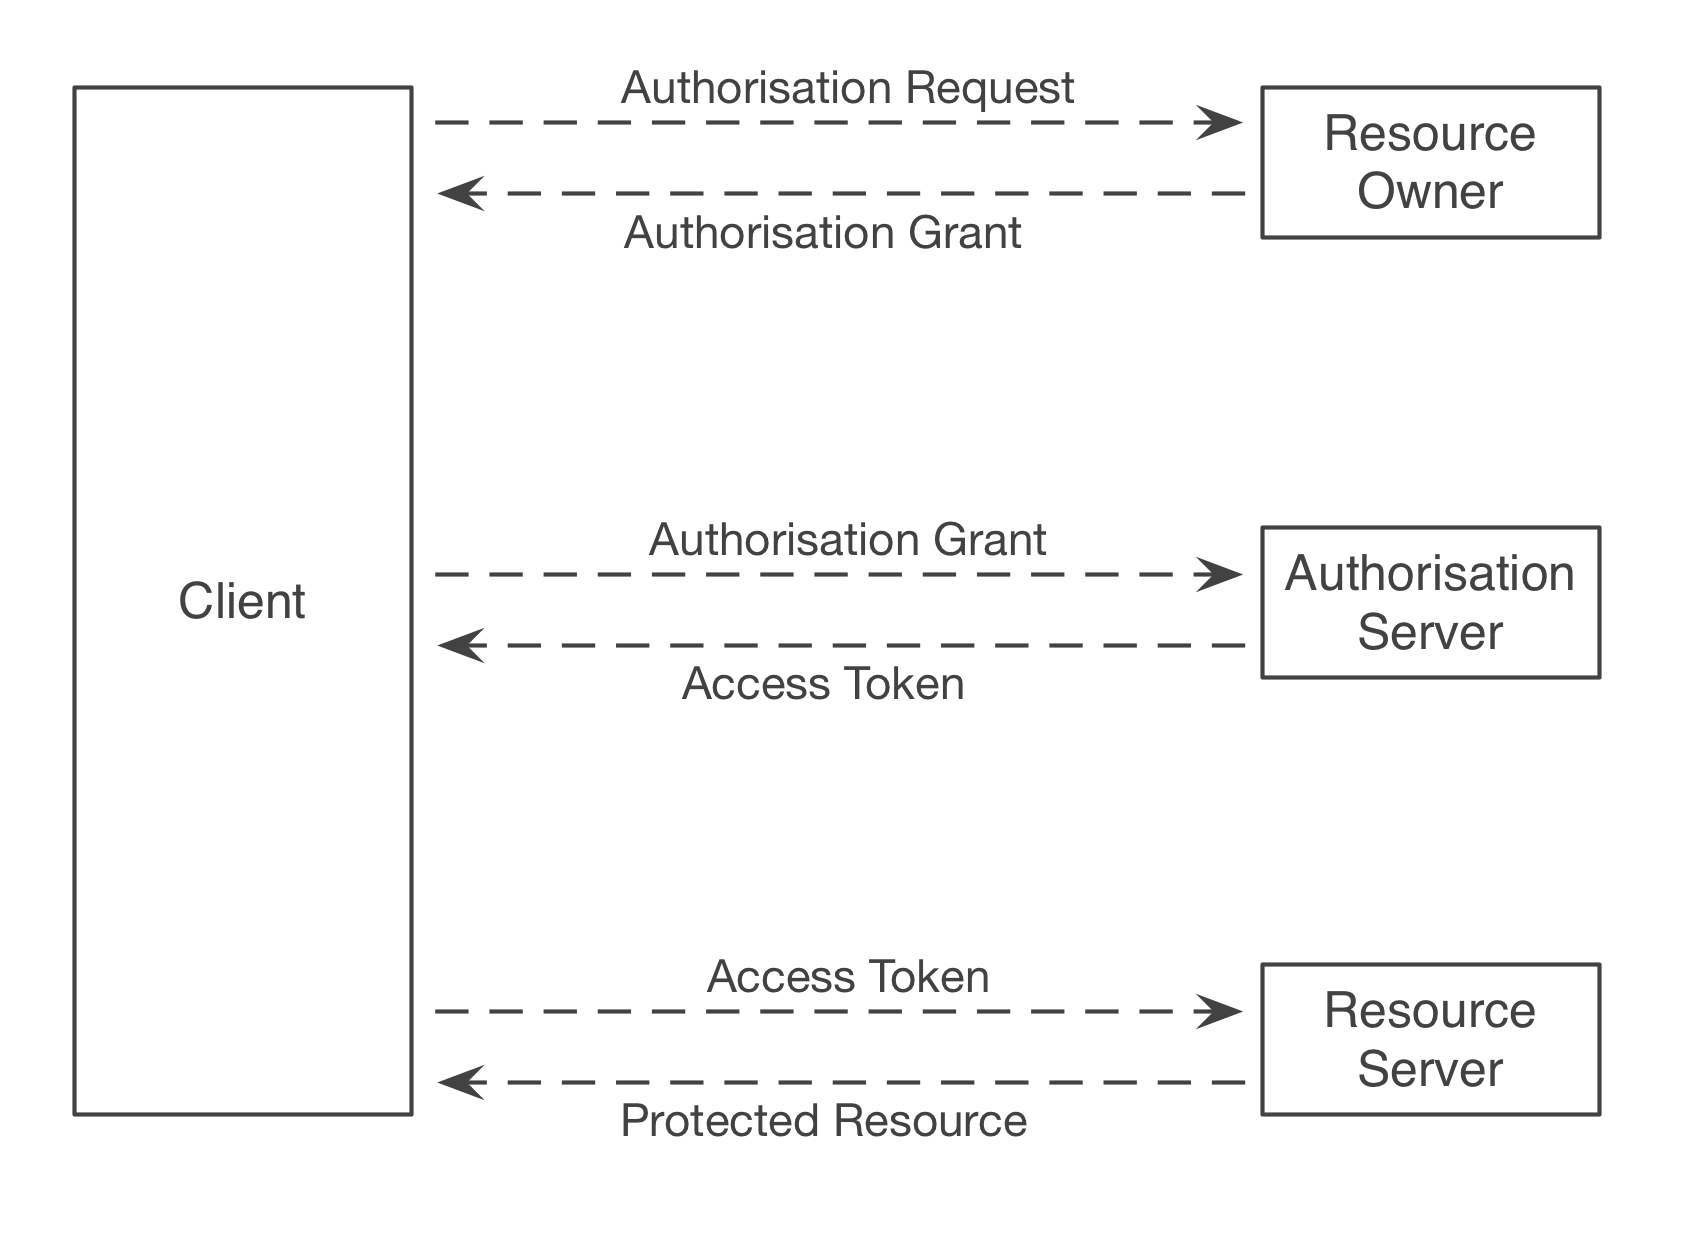
\includegraphics[width=\textwidth]{figures/OAuth2Flow.png}
\caption[OAuth 2.0 Flow.]{The abstract OAuth 2.0 flow describes the interaction between the four roles within the defined steps.
\label{fig:oauth2flow}}
\end{figure}

The six steps in the abstract OAuth 2.0 flow are defined as follows:
\begin{enumerate}
    \item The client sends an authorisation request to the resource owner, either directly or via the authorisation server as intermediary.
    \item The client receives an authorisation grant.
    \item The client requests an access token by presenting the authorisation grant.
    \item The client is authenticated by the authorisation server which issues and access token.
    \item The client now requests the protected resource presenting the access token.
    \item The resource server validates the token and replies with the resource representation if valid.
\end{enumerate}

JSON Web Token (JWT)~\cite{jones2015json} is a compact, URL-safe mechanism to represent and transfer claims between two parties. The claims are encoded as a JSON object. This can be used as the payload of a JSON Web Signature (JWS)~\cite{jones2014n} structure, or as the plaintext in a JSON Web Encryption~\cite{jones2015jwe} structure. Therefore, JWT allows for the claims to be digitally signed or integrity protected integrity protected with a Message Authentication Code (MAC) and/or encrypted.

\subsection{Scenarios}

We consider a scenario in which a user wants to log-in to a SP without having to directly expose their identity, by leveraging with an IdP. Both the user and the SP trust the IdP. In this scenario we have three parties:
\begin{itemize}
    \item client
    \item service
    \item identity provider
\end{itemize}

Before starting an authentication and subsequent authorisation process the client needs to create an identity on the IdP. This step can be consider as an \emph{initialisation} phase.

\subsection{Account creation on the IdP}

To create an account on the IdP we assume that as the client is initialised it will generate a number of cryptographic keys to authenticate the various user identities. The keys can be saved in a wallet and used to register identities on the IdP. A use might decide to use different keys for each service or the same key for a group of services. Note that each key doesn't correspond to a service account Id. A key is actually an account identification for the IdP which is stored and used by the client.

To create an account on a service the client prepares a request for the IdP performing a set of cryptographic operations that allows the client to register an anonymous identifier for the service. To implement such algorithm, we need a
cryptographically secure hash function and a secure elliptic curve group. JSON Web Algorithms (JWA)~\cite{jones2015jwa}, provides Hash-based Message Authentication Codes (HMACs). HMACs enable the client to compute a MAC from a secret (the user's key) plus a cryptographic hash function. The algorithm for implementing and validating HMACs is provided in RFC 2104~\cite{krawczyk1997rfc}.

The account can be completely anonymous on the IdP side as long as the SP is able to eventually blacklist the account in case they perform some malicious action.
 
\subsection{Authorisation request on WebSocket}

We imagine that a client has already established a handshake request with a server over WebSocket and is waiting to establish a communication. In this case the client will initiate an authorization process with the server where it wants to prove that it knows a the secret pseudonym registered with the server.

In this case, the client will initiate the Socialist Millionaires protocol to prove the server they know the pseudonym.

Imagine that a \emph{Prover} (the client) wants to prove the \emph{Verifier} (the server) that they know a certain pseudonym. Given a known elliptic curve $C$, a generator for such curve $G$ and the curve order the protocol can be outlined as follows:

The Prover initiate the process and sends an authorisation request by transmitting the result of a certain computation:
\begin{enumerate}
    \item Prover picks two random numbers: $a2$ and $a3$.
    \item Prover computes $G2a = a2 * G$ and $G3a = a3 * G$.
    \item Prover transmits $G2a$ and $G3a$ to the Verifier.
\end{enumerate}

The Verifier received the two values initiate the authorisation process on their side:
\begin{enumerate}
    \item Verifier picks two random numbers: $b2$ and $b3$. 
    \item Verifier computes $G2b = b2 * G$ and $G3b = b3 * G$.
    \item Verifier computes $G2B = b2 * G2a$ and $G3B = b3 * G3a$.
    \item Verifier picks random number $r$.
    \item Verifier computes $Pb = r * G3B$ and $Qb = r * G + y * G2B$.
    \item Verifier transmits $G2b$, $G3b$, $Pb$ and $Qb$ to Prover.
\end{enumerate}

The Prover receives the first answer from the Verifier and continues the protocol:
\begin{enumerate}
    \item Prover computes $G2A = a2 * G2b$ and $G3A = a3 * G3b$.
    \item Prover picks random number $s$.
    \item Prover computes $Pa = s * G3A$ and $Qa = s * G + x * G2A$.
    \item Prover computes $Ra = a3 * (Qa - Qb)$.
    \item Prover transmits $Pa$, $Qa$, $Ra$ to Verifier.
\end{enumerate}

Now the Verifier will compute the proof with the values received and ultimately transmitt the results of their computation to the Prover authorising the data transfer:
\begin{enumerate}
    \item Verifier computes $Rb = b3 * (Qa - Qb)$.
    \item Verifier computes $Rba = b3 * Ra$.
    \item Verifier checks that $Rab == Pa - Pb$.
\end{enumerate}

Now the Prover will verify the result on their side by performing the following computations:

\begin{enumerate}
    \item Prover computes $Rab = a3 * Rb$.
    \item Prover checks whether $Rab == Pa - Pb$.
\end{enumerate}

Now the client can also initiate the data transfer to disclose information or receive an authorisation ticket that can be used with a third party.

\subsection{Authorisation request on OAuth}

A possible OAuth flow can be described as follows (Figure ~\ref{fig:privateflow}):
\begin{enumerate}
    \item The client sends an authorisation request to the IdP. This request is signed and encrypted and packed into a JWT.
    \item If the request is valid the IdP issues a token.
    \item The client uses the token to authenticate with the service. Which is verified separately with the IdP.
    \item The service returns access to the protected resource through its representation.
\end{enumerate}

\begin{figure}
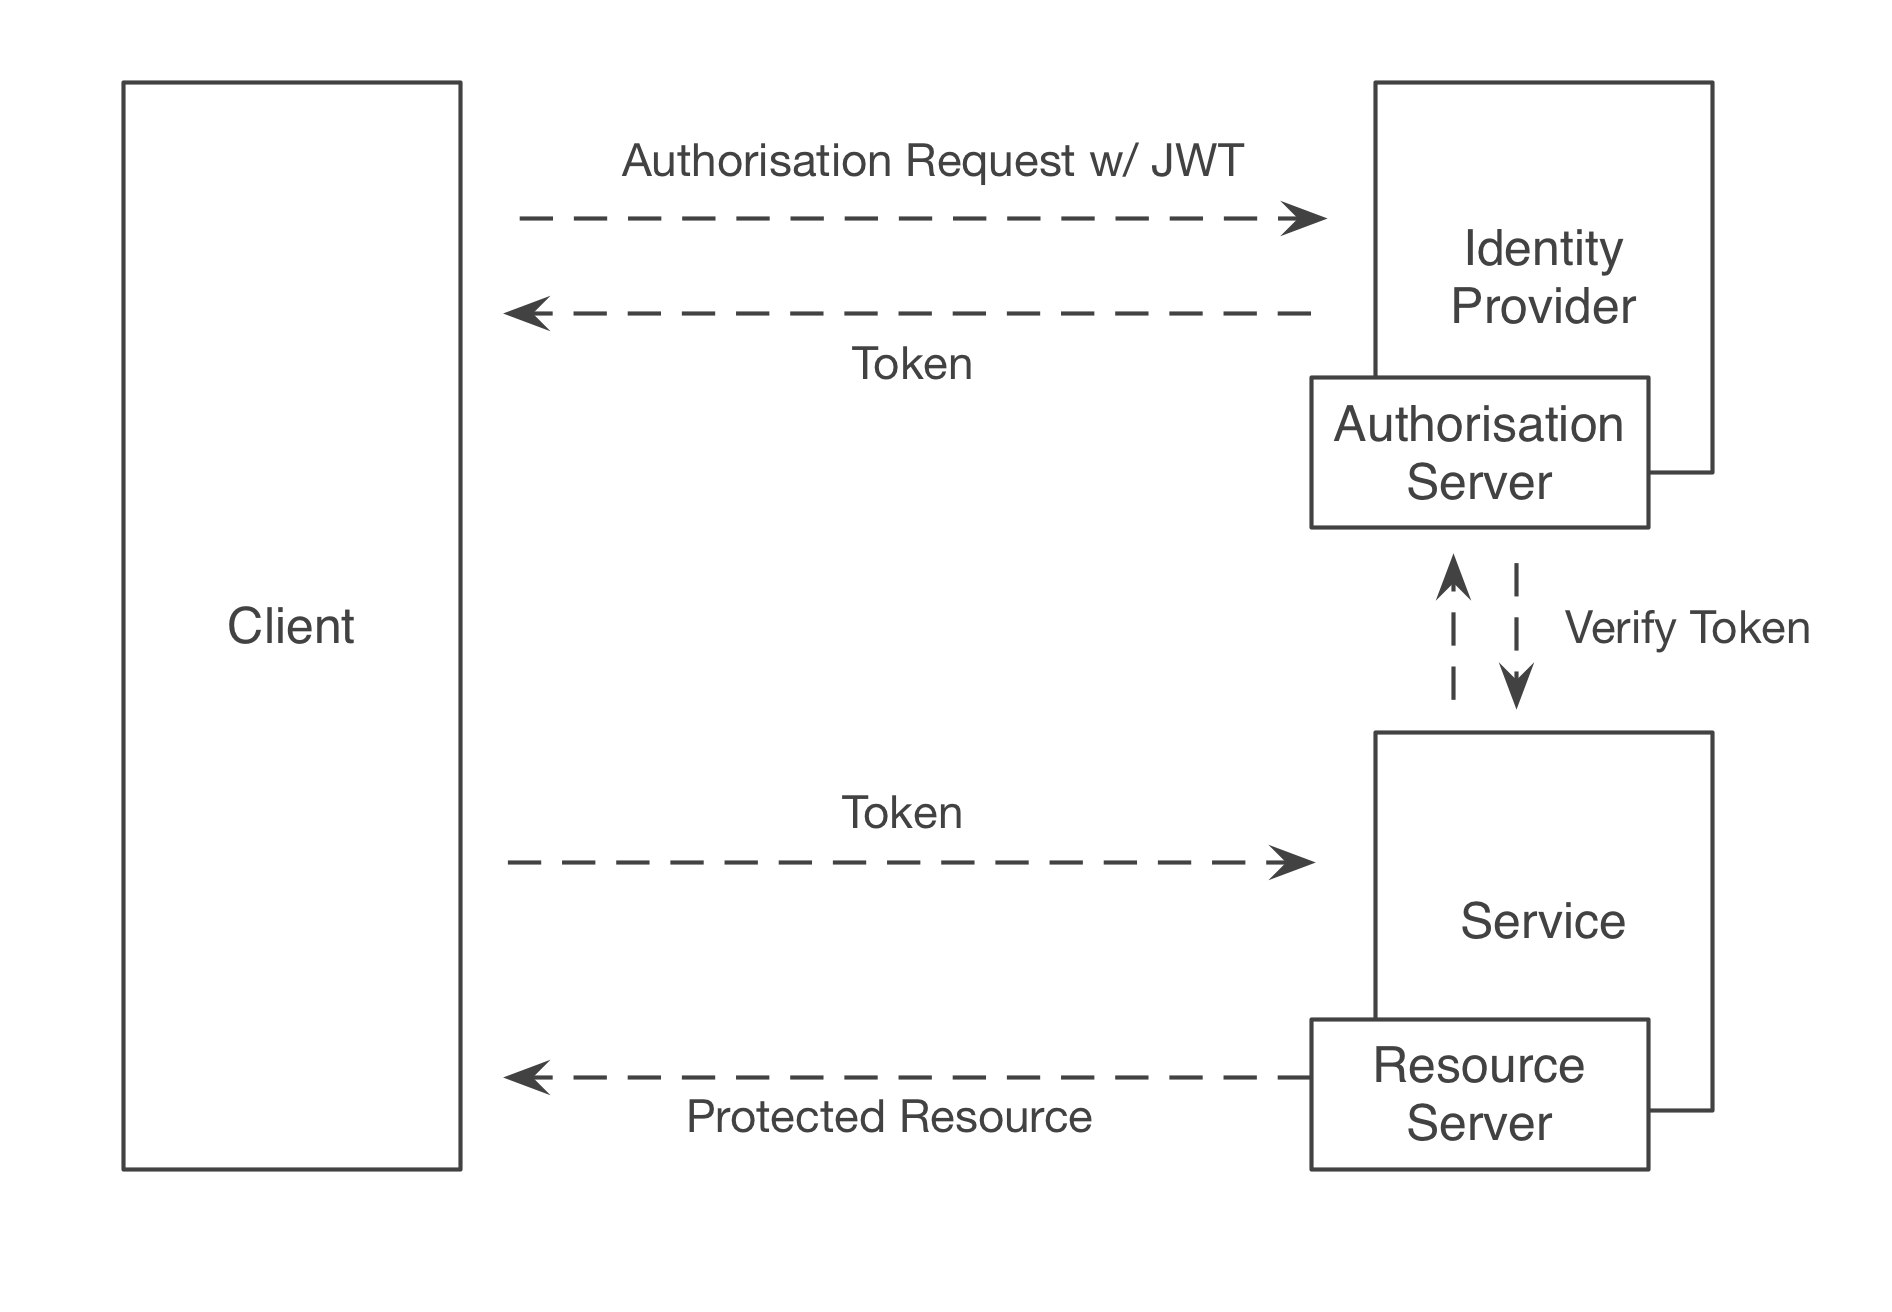
\includegraphics[width=\textwidth]{figures/PrivateFlow.png}
\caption[Privacy Preserving OAuth Flow with JWT.]{The privacy preserving OAuth 2 flow uses JWT to transmit user information.
\label{fig:privateflow}}
\end{figure}

Once the client is issued a \emph{token} from the IdP it can authenticate with the \emph{service}. Hence, the issued \emph{token} which encodes the claims and service id can be transmitted to the service encrypted with the JWE protocol. The token can then be verified and the client authorised to request the protected resource. An account is created on the service if the authentication protocol is initiated for the first time.

\subsection{Protocol description}

The protocol flow was implemented as follows:
\begin{enumerate}
    \item The client sends an authorisation request to the IdP.
    \item The client receives an authorisation grant via a \emph{JWT} encoding the 0-knowledge proof to present to the SP.
    \item The client engages the SP in a zero-knowledge proof that it holds a valid credential from the IdP.
    \item The client is authenticated (or not).
    \item The client can now request protected resources, or the SP can request further information from the client.
\end{enumerate}

JWE is used within JWTs to encrypt content using JSON data structures and base64url encoding.

A JWE includes the following logical fields:
\begin{itemize}
    \item JOSE Header
    \item JWE Encrypted Key
    \item JWE Initialization Vector
    \item JWE AAD
    \item JWE Ciphertext
    \item JWE Authentication Tag
\end{itemize}

Furthermore the JOSE Header is a field composed of the following fields:
\begin{itemize}
    \item JWE Protected Header
    \item JWE Shared Unprotected Header
    \item JWE Per-Recipient Unprotected Header
\end{itemize}

To perform operation regarding Message Authentication Codes (MACs) or secure content with digital signatures, we can use JSON Web Signature (JWS) provided by JWA. The JWS cryptographic mechanisms provide integrity protection for an arbitrary sequence of octets.  

A JWS object can be created following the syntax below:
\lstset{caption={An example of a JWS object.},label=lst:payload}
\begin{lstlisting}
     {
      "payload":"<payload contents>",
      "signatures":[
       {"protected":"<integrity-protected header 1 contents>",
        "header":<non-integrity-protected header 1 contents>,
        "signature":"<signature 1 contents>"},
       ...
       {"protected":"<integrity-protected header N contents>",
        "header":<non-integrity-protected header N contents>,
        "signature":"<signature N contents>"}]
     }

\end{lstlisting}

The client can prove to know the secret pseudonym by solving a cryptographic challenge in the request over oauth to the server, given a secure cryptographic curve and its generator $G$ and it's order $q$. More specifically the server stores an encrypted version of the pseudonym as $Q = x * G$, therefore the client can prove that they know $0 < x < q$ such that $Q = x * G$ by:
\begin{enumerate}
    \item Computing $Q = x * G$.
    \item Picking a random number $r$.
    \item Computing $c = HASH(r * G)$.
    \item Computing $d = r - x*c mod q$
    \item Transmitting (c,d) to the server over a JWT.
\end{enumerate}

The server will prove that $c == HASH(d * G + c * Q)$ and issue a JWT with an authorisation ticket.
The client can use the ticket to disclose information with the IdP. The Idp can use the disclosed information to sing a statement to the SP regarding the client without disclosing the information or can authorise the client to access the SP by voucing for them.

\section{Privacy management}

The protocol flow described up to this point allows the client to granularly disclose information to the SP. More importantly in the current federated log in mechanism, implemented by IdPs like Facebook, third-party apps can always request to the IdP updated information regarding the user. With the proposed mechanism, third-party apps will have to request the information to the client, that can refuse to provide them or can provide different values depending on the context. 
We believe this aspect is fundamental for implementing Privacy Management Technologies without having to change the way users interact with web apps and without having to change existing web protocols that are so widely adopted. Up to now, privacy enhancement and privacy management solution have been focusing with the network level of the user's communications. This approach instead shift the focus to client interactions and existing web protocols that can be used and eventually improved to support such techniques.

\section{Prototype evaluation}

Implementation of the protocols described are available in various programming languages, as are considered industry standards. We tested the protocol described with the EdDSA implementation provided by ECPy~\cite{ecpy}, a pure python Elliptic Curve library providing ECDSA, EDDSA, ECSchnorr, Borromean signatures as well as Point operations.

The implementation for the Socialist Millionaire Protocol takes 187 lines of codes in total and takes 0.05619168281555176 seconds to run on a Intel Core i7-6600U CPU @ 2.60GHz × 4 cores. On the other hand, the implementation with the same libraries for the challenge implemented in the OAuth example takes only 20 line of code and takes 0.031212568283081055 seconds to run on the same machine.

\section{Discussion}

The example illustrated above show how web applications can be easily patched to provide users with a more privacy friendly experience. Up to now, in fact, users have been given the choice to either accept the terms of SPs and share all the data requested or not use the service. The model proposed instead would give users control on how they can share the data and present SPs with certain information regarding the users. 
Furthermore, SPs will not be given the possibility to access user information from the IdP as they please, but will have to request users to disclose certain information to the IdP. This way users will know exactly which information has been disclosed and in which interaction with SPs, hence giving them the choice to request for the data to be deleted if they wished to do so.
We believe this to be an important paradigm change in the way authentication and authorisation with SPs is implemented and a much needed improvement for privacy management on the client side.
